%%%%%%%%%%%%%%%%%%%%%%%%%%%%%%%%%%%%%%%%
% datoteka diploma-vzorec.tex
%
% vzorčna datoteka za pisanje diplomskega dela v formatu LaTeX
% na UL Fakulteti za računalništvo in informatiko
%
% vkup spravil Gašper Fijavž, december 2010
% 
%
%
% verzija 12. februar 2014 (besedilo teme, seznam kratic, popravki Gašper Fijavž)
% verzija 10. marec 2014 (redakcijski popravki Zoran Bosnić)
% verzija 11. marec 2014 (redakcijski popravki Gašper Fijavž)
% verzija 15. april 2014 (pdf/a 1b compliance, not really - just claiming, Damjan Cvetan, Gašper Fijavž)
% verzija 23. april 2014 (privzeto cc licenca)
% verzija 16. september 2014 (odmiki strain od roba)
% verzija 28. oktober 2014 (odstranil vpisno številko)
% verija 5. februar 2015 (Literatura v kazalu, online literatura)
% verzija 25. september 2015 (angl. naslov v izjavi o avtorstvu)
% verzija 26. februar 2016 (UL izjava o avtorstvu)
% verzija 16. april 2016 (odstranjena izjava o avtorstvu)
% verzija 5. junij 2016 (Franc Solina dodal vrstice, ki jih je označil s svojim imenom)


\documentclass[a4paper, 12pt]{book}
%\documentclass[a4paper, 12pt, draft]{book}  Nalogo preverite tudi z opcijo draft, ki vam bo pokazala, katere vrstice so predolge!



\usepackage[utf8x]{inputenc}   % omogoča uporabo slovenskih črk kodiranih v formatu UTF-8
\usepackage[slovene,english]{babel}    % naloži, med drugim, slovenske delilne vzorce
\usepackage[pdftex]{graphicx}  % omogoča vlaganje slik različnih formatov
\usepackage{fancyhdr}          % poskrbi, na primer, za glave strani
\usepackage{amssymb}           % dodatni simboli
\usepackage{amsmath}           % eqref, npr.
%\usepackage{hyperxmp}
\usepackage[hyphens]{url}  % dodal Solina
\usepackage{comment}       % dodal Solina

\usepackage[pdftex, colorlinks=true,
						citecolor=black, filecolor=black, 
						linkcolor=black, urlcolor=black,
						pagebackref=false, 
						pdfproducer={LaTeX}, pdfcreator={LaTeX}, hidelinks]{hyperref}

\usepackage{color}       % dodal Solina
\usepackage{soul}       % dodal Solina

%%%%%%%%%%%%%%%%%%%%%%%%%%%%%%%%%%%%%%%%
%	DIPLOMA INFO
%%%%%%%%%%%%%%%%%%%%%%%%%%%%%%%%%%%%%%%%
\newcommand{\ttitle}{Učenje realno-časovne strateške igre z uporabo globokega spodbujevalnega učenja}
\newcommand{\ttitleEn}{Teaching of real-time strategy game using deep reinforcement learning}
\newcommand{\tsubject}{\ttitle}
\newcommand{\tsubjectEn}{\ttitleEn}
\newcommand{\tauthor}{Jernej Habjan}
\newcommand{\tkeywords}{Alpha Zero, realno-časovna strateška igra, Unreal Engine}
\newcommand{\tkeywordsEn}{Alpha Zero, real-time strategy game, Unreal Engine}


%%%%%%%%%%%%%%%%%%%%%%%%%%%%%%%%%%%%%%%%
%	HYPERREF SETUP
%%%%%%%%%%%%%%%%%%%%%%%%%%%%%%%%%%%%%%%%
\hypersetup{pdftitle={\ttitle}}
\hypersetup{pdfsubject=\ttitleEn}
\hypersetup{pdfauthor={\tauthor, jh0228@student.uni-lj.si}}
\hypersetup{pdfkeywords=\tkeywordsEn}


 


%%%%%%%%%%%%%%%%%%%%%%%%%%%%%%%%%%%%%%%%
% postavitev strani
%%%%%%%%%%%%%%%%%%%%%%%%%%%%%%%%%%%%%%%%  

\addtolength{\marginparwidth}{-20pt} % robovi za tisk
\addtolength{\oddsidemargin}{40pt}
\addtolength{\evensidemargin}{-40pt}

\renewcommand{\baselinestretch}{1.3} % ustrezen razmik med vrsticami
\setlength{\headheight}{15pt}        % potreben prostor na vrhu
\renewcommand{\chaptermark}[1]%
{\markboth{\MakeUppercase{\thechapter.\ #1}}{}} \renewcommand{\sectionmark}[1]%
{\markright{\MakeUppercase{\thesection.\ #1}}} \renewcommand{\headrulewidth}{0.5pt} \renewcommand{\footrulewidth}{0pt}
\fancyhf{}
\fancyhead[LE,RO]{\sl \thepage} 
%\fancyhead[LO]{\sl \rightmark} \fancyhead[RE]{\sl \leftmark}
\fancyhead[RE]{\sc \tauthor}              % dodal Solina
\fancyhead[LO]{\sc Diplomska naloga}     % dodal Solina


\newcommand{\BibTeX}{{\sc Bib}\TeX}

%%%%%%%%%%%%%%%%%%%%%%%%%%%%%%%%%%%%%%%%
% naslovi
%%%%%%%%%%%%%%%%%%%%%%%%%%%%%%%%%%%%%%%%  


\newcommand{\autfont}{\Large}
\newcommand{\titfont}{\LARGE\bf}
\newcommand{\clearemptydoublepage}{\newpage{\pagestyle{empty}\cleardoublepage}}
\setcounter{tocdepth}{1}	      % globina kazala

%%%%%%%%%%%%%%%%%%%%%%%%%%%%%%%%%%%%%%%%
% konstrukti
%%%%%%%%%%%%%%%%%%%%%%%%%%%%%%%%%%%%%%%%  
\newtheorem{izrek}{Izrek}[chapter]
\newtheorem{trditev}{Trditev}[izrek]
\newenvironment{dokaz}{\emph{Dokaz.}\ }{\hspace{\fill}{$\Box$}}

%%%%%%%%%%%%%%%%%%%%%%%%%%%%%%%%%%%%%%%%%%%%%%%%%%%%%%%%%%%%%%%%%%%%%%%%%%%%%%%
%% PDF-A
%%%%%%%%%%%%%%%%%%%%%%%%%%%%%%%%%%%%%%%%%%%%%%%%%%%%%%%%%%%%%%%%%%%%%%%%%%%%%%%


%%%%%%%%%%%%%%%%%%%%%%%%%%%%%%%%%%%%%%%% 
% define medatata
%%%%%%%%%%%%%%%%%%%%%%%%%%%%%%%%%%%%%%%% 
\def\Title{\ttitle}
\def\Author{\tauthor, jh0228@student.uni-lj.si}
\def\Subject{\ttitleEn}
\def\Keywords{\tkeywordsEn}

%%%%%%%%%%%%%%%%%%%%%%%%%%%%%%%%%%%%%%%% 
% \convertDate converts D:20080419103507+02'00' to 2008-04-19T10:35:07+02:00
%%%%%%%%%%%%%%%%%%%%%%%%%%%%%%%%%%%%%%%% 
\def\convertDate{%
    \getYear
}

{\catcode`\D=12
 \gdef\getYear D:#1#2#3#4{\edef\xYear{#1#2#3#4}\getMonth}
}
\def\getMonth#1#2{\edef\xMonth{#1#2}\getDay}
\def\getDay#1#2{\edef\xDay{#1#2}\getHour}
\def\getHour#1#2{\edef\xHour{#1#2}\getMin}
\def\getMin#1#2{\edef\xMin{#1#2}\getSec}
\def\getSec#1#2{\edef\xSec{#1#2}\getTZh}
\def\getTZh +#1#2{\edef\xTZh{#1#2}\getTZm}
\def\getTZm '#1#2'{%
    \edef\xTZm{#1#2}%
    \edef\convDate{\xYear-\xMonth-\xDay T\xHour:\xMin:\xSec+\xTZh:\xTZm}%
}

\expandafter\convertDate\pdfcreationdate 

%%%%%%%%%%%%%%%%%%%%%%%%%%%%%%%%%%%%%%%%
% get pdftex version string
%%%%%%%%%%%%%%%%%%%%%%%%%%%%%%%%%%%%%%%% 
\newcount\countA
\countA=\pdftexversion
\advance \countA by -100
\def\pdftexVersionStr{pdfTeX-1.\the\countA.\pdftexrevision}


%%%%%%%%%%%%%%%%%%%%%%%%%%%%%%%%%%%%%%%%
% XMP data
%%%%%%%%%%%%%%%%%%%%%%%%%%%%%%%%%%%%%%%%  
\usepackage{xmpincl}
\includexmp{pdfa-1b}

%%%%%%%%%%%%%%%%%%%%%%%%%%%%%%%%%%%%%%%%
% pdfInfo
%%%%%%%%%%%%%%%%%%%%%%%%%%%%%%%%%%%%%%%%  
\pdfinfo{%
    /Title    (\ttitle)
    /Author   (\tauthor, damjan@cvetan.si)
    /Subject  (\ttitleEn)
    /Keywords (\tkeywordsEn)
    /ModDate  (\pdfcreationdate)
    /Trapped  /False
}


%%%%%%%%%%%%%%%%%%%%%%%%%%%%%%%%%%%%%%%%%%%%%%%%%%%%%%%%%%%%%%%%%%%%%%%%%%%%%%%
%%%%%%%%%%%%%%%%%%%%%%%%%%%%%%%%%%%%%%%%%%%%%%%%%%%%%%%%%%%%%%%%%%%%%%%%%%%%%%%

\begin{document}
\selectlanguage{slovene}
\frontmatter
\setcounter{page}{1} %
\renewcommand{\thepage}{}       % preprecimo težave s številkami strani v kazalu
\newcommand{\sn}[1]{"`#1"'}                    % dodal Solina (slovenski narekovaji)

%%%%%%%%%%%%%%%%%%%%%%%%%%%%%%%%%%%%%%%%
%naslovnica
 \thispagestyle{empty}%
   \begin{center}
    {\large\sc Univerza v Ljubljani\\%
      Fakulteta za računalništvo in informatiko}%
    \vskip 10em%
    {\autfont \tauthor\par}%
    {\titfont \ttitle \par}%
    {\vskip 3em \textsc{DIPLOMSKO DELO\\[5mm]         % dodal Solina za ostale študijske programe
%    VISOKOŠOLSKI STROKOVNI ŠTUDIJSKI PROGRAM\\ PRVE STOPNJE\\ RAČUNALNIŠTVO IN INFORMATIKA}\par}%
    UNIVERZITETNI  ŠTUDIJSKI PROGRAM\\ PRVE STOPNJE\\ RAČUNALNIŠTVO IN INFORMATIKA}\par}%
%    INTERDISCIPLINARNI UNIVERZITETNI\\ ŠTUDIJSKI PROGRAM PRVE STOPNJE\\ RAČUNALNIŠTVO IN MATEMATIKA}\par}%
%    INTERDISCIPLINARNI UNIVERZITETNI\\ ŠTUDIJSKI PROGRAM PRVE STOPNJE\\ UPRAVNA INFORMATIKA}\par}%
%    INTERDISCIPLINARNI UNIVERZITETNI\\ ŠTUDIJSKI PROGRAM PRVE STOPNJE\\ MULTIMEDIJA}\par}%
    \vfill\null%
    {\large \textsc{Mentor}: doc.\ dr. Matej Guid\par}%
   {\large \textsc{Somentor}:  prof.\ dr. Branko Šter \par}%
    {\vskip 2em \large Ljubljana, 2018 \par}%
\end{center}
% prazna stran
%\clearemptydoublepage      % dodal Solina (izjava o licencah itd. se izpiše na hrbtni strani naslovnice)

%%%%%%%%%%%%%%%%%%%%%%%%%%%%%%%%%%%%%%%%
%copyright stran
\thispagestyle{empty}
\vspace*{8cm}

\noindent
{\sc Copyright}. 
Rezultati diplomske naloge so intelektualna lastnina avtorja in Fakultete za računalništvo in informatiko Univerze v Ljubljani.
Za objavo in koriščenje rezultatov diplomske naloge je potrebno pisno privoljenje avtorja, Fakultete za računalništvo in informatiko ter mentorja.

\begin{center}
\mbox{}\vfill
\emph{Besedilo je oblikovano z urejevalnikom besedil \LaTeX.}
\end{center}
% prazna stran
\clearemptydoublepage

%%%%%%%%%%%%%%%%%%%%%%%%%%%%%%%%%%%%%%%%
% stran 3 med uvodnimi listi
\thispagestyle{empty}
\vspace*{4cm}

\noindent
Fakulteta za računalništvo in informatiko izdaja naslednjo nalogo:
\medskip
\begin{tabbing}
\hspace{32mm}\= \hspace{6cm} \= \kill




Tematika naloge:
\end{tabbing}
Besedilo teme diplomskega dela študent prepiše iz študijskega informacijskega sistema, kamor ga je vnesel mentor. V nekaj stavkih bo opisal, kaj pričakuje od kandidatovega diplomskega dela. Kaj so cilji, kakšne metode uporabiti, morda bo zapisal tudi ključno literaturo.
\vspace{15mm}






\vspace{2cm}

% prazna stran
\clearemptydoublepage

% zahvala
\thispagestyle{empty}\mbox{}\vfill\null\it%
\noindent
Zahvaljujem se mentorju doc.\ dr. Mateju Guidu in somentorju prof.\ dr. Branku Šteru, prijateljem in družini, ki so mi pomagali pri pisanju diplomske naloge.
\rm\normalfont

% prazna stran
\clearemptydoublepage


% kazalo
\pagestyle{empty}
\def\thepage{}% preprecimo tezave s stevilkami strani v kazalu
\tableofcontents{}


% prazna stran
\clearemptydoublepage

%%%%%%%%%%%%%%%%%%%%%%%%%%%%%%%%%%%%%%%%
% seznam kratic

\chapter*{Seznam uporabljenih kratic}  % spremenil Solina, da predolge vrstice ne gredo preko desnega roba

\begin{comment}
\begin{tabular}{l|l|l}
  {\bf kratica} & {\bf angleško} & {\bf slovensko} \\ \hline
  % after \\: \hline or \cline{col1-col2} \cline{col3-col4} ...
  {\bf CA} & classification accuracy & klasifikacijska točnost \\
  {\bf DBMS} & database management system & sistem za upravljanje podatkovnih baz \\
  {\bf SVM} & support vector machine & metoda podpornih vektorjev \\
  \dots & \dots & \dots \\
\end{tabular}
\end{comment}

\noindent\begin{tabular}{p{0.1\textwidth}|p{.4\textwidth}|p{.4\textwidth}}    % po potrebi razširi prvo kolono tabele na račun drugih dveh!
  {\bf kratica} & {\bf angleško}                             & {\bf slovensko} \\ \hline
   {\bf MCTS}      & Monte Carlo tree search               & Monte-Carlo drevesno preiskovanje \\
  {\bf UE4} & game engine Unreal Engine 4 & celostni pogon Unreal Engine 4 \\
  {\bf RTS} & real-time strategy & realno-časovna strateška \\
\end{tabular}


% prazna stran
\clearemptydoublepage

%%%%%%%%%%%%%%%%%%%%%%%%%%%%%%%%%%%%%%%%
% povzetek
\addcontentsline{toc}{chapter}{Povzetek}
\chapter*{Povzetek}

\noindent\textbf{Naslov:} \ttitle
\bigskip

\noindent\textbf{Avtor:} \tauthor
\bigskip

%\noindent\textbf{Povzetek:} 
\noindent 
Z obstoječim Alpha Zero algoritmom smo implementirali učenje in priporočanje akcij v realno-časovni strateški igri.
Pregledali smo krajšo zgodovino globokega spodbujevalnega učenja na igrah in povzeli zakaj je pristop samostojnega učenja najprimernejši.
Za strateško igro smo definirali figure in njihove akcije in zakodirali kompleksno stanje igre s kodirnikom.
Prav tako smo definirali ustavitvene pogoje pri igri, ki nima končnega števila potez na podlagi poškodovanja figur.
Rezultate smo prikazali s Python modulom Pygame in v celostnem pogonu Unreal Engine 4. 
V obeh vizualizacijah lahko igramo proti naučenem modelu, ali pa opazujemo, kako se dva računalniška nasprotnika bojujeta med sabo.
Na koncu smo še pregledali rezultate in povzeli učinek učenja algoritma.
\bigskip

\noindent\textbf{Ključne besede:} \tkeywords.
% prazna stran
\clearemptydoublepage

%%%%%%%%%%%%%%%%%%%%%%%%%%%%%%%%%%%%%%%%
% abstract
\selectlanguage{english}
\addcontentsline{toc}{chapter}{Abstract}
\chapter*{Abstract}

\noindent\textbf{Title:} \ttitleEn
\bigskip

\noindent\textbf{Author:} \tauthor
\bigskip

%\noindent\textbf{Abstract:} 
\noindent With the existing Alpha Zero algorithm, we implemented learning and recommending actions in a real-time strategy game.
We examined the shorter history of deep stimulating learning in games and summarized why the self-learning approach is most appropriate.
For a strategic game, we defined the figures and their actions and encoded the complex state of the game with the encoder.
We also defined the stopping conditions of the game, which has no final number of moves based on damage to the figures.
The results were displayed with the Python Pygame module and the Unreal Engine 4 integrated drive.
In both visualizations we can play against the learned model, or we can observe how two computer opponents are fighting each other.
In the end, we have also reviewed the results and summarized the learning effect of the algorithm.
\bigskip

\noindent\textbf{Keywords:} \tkeywordsEn.
\selectlanguage{slovene}
% prazna stran
\clearemptydoublepage

%%%%%%%%%%%%%%%%%%%%%%%%%%%%%%%%%%%%%%%%
\mainmatter
\setcounter{page}{1}
\pagestyle{fancy}

\chapter{Uvod}


Razvijanje inteligentnega agenta v realno-časovnih oziroma RTS igrah je problem, s katerim se mora soočiti večina razvijalcev teh iger, agentove akcije so pa pogosto predvidljive, saj se človeški igralec nauči njihovih načinov delovanja in jih tako lažje premaga.
Če pustimo agentu, da sam opravlja akcije nekontrolirano, bo izvajal naključne akcije, ki so pa slabše kot vnaprej definirana taktika.
Če pa agentu podamo hevristiko, po kateri se mora ravnati, bo poskušal izvesti čim boljšo akcijo, vendar bo za njen izračun porabil predolgo časa, saj bo moral preiskati cel preiskovalni prostor, ki pa pri realno-časovnih strateških igrah zna biti prevelik.
Na primer 10 enot v igri, kjer ima vsaka 5 možnih potez, se razveji na možen faktor $5^{10}$ ≈ 10 milijonov možnih akcij.
Za igro StarCraft je ocenjenih možnih vsaj $10^{1685}$ možnih akcij, kjer je za šah $10^{47}$ in $10^{171}$ za igro Go~\cite{ontanon2017combinatorial}.

Preiskovanje prostora z grobo silo torej odpade. 
Ostanejo nam potem hevristični algoritmi, kot so Alpha-Beta rezanje ali Monte-Carlo drevesno preiskovanje oziroma MCTS. 
Ampak Alpha-Beta deluje dobro samo pod pogoji, da obstaja zanesljiva evaluacijska funkcija in da ima igra majhen vejitveni prostor, kar je pa lastnost veliko klasičnih namiznih iger kot Go in video iger. Zato se je bolje v takih primerih odločiti za MCTS~\cite{chaslot2008monte}.
MCTS pa ima pomanjkljivost, da si stanj igre ne zapomni skozi več iger, kjer bi lahko to vrednost stanja uporabil za bolj natančen izračun naslednjih stanj.

Za memorizacijo stanj pa pridejo v upoštev globoke nevronske mreže, ki pa z učenjem ugotovijo zakonitosti v učni množici in skozi mnogo iteracij izboljšajo svojo predikcijo določenega izhoda ob določenem vhodu. To je pa točno to, kar potrebuje MCTS kot začetno stanje, iz katerega lažje izračuna najboljšo akcijo.

Da pa nevronska mreža dobi dovolj vhodnih podatkov za učenje, pa moramo realizirati algoritem, ki bo igral proti drugem računalniškem nasprotniku, in pridobil rezultat, ali je to igro zmagal, ali zgubil. 
Ob tem izhodu nevronska mreža nagradi svoje predikcije ob določenem stanju, ali pa jih kaznuje.

To je glavna ideja o implementaciji algoritma, ki jo pa vsebuje algoritem Alpha Zero, ki smo ga uporabili v tej diplomski nalogi.
Algoritem se nauči igranja igre z igranjem iger sam proti sebi, kjer boljša različica algoritma napreduje v naslednji krog.
Ko je model nevronske mreže naučen, ga lahko uporabimo, da nam priporoči akcijo v določenem stanju.
Tako lahko implementiramo računalniškega igralca, ki pridobiva akcije od naučenega modela in jih izvršuje, kot tudi priporočilni sistem za akcije, ki jih prikazujemo človeškemu igralcu. Algoritem nam priporoči akcijo in ne tipa strategije, katerega naj izberemo, kar bi potrebovalo še bolj abstrakten pogled na igro. 

O strateških igrah, njihovih abstrakcijah in zakaj so tako zanimive za raziskovanje umetne inteligence bomo več spoznali v poglavju \ref{chrts}.
V poglavju \ref{alphazero} bomo podrobneje pregledali sestavo Alpha Zero algoritma in zakaj je primeren za našo RTS igro.
Ko bomo imeli sestavljen algoritem, bomo zanj sestavili RTS igro v poglavju \ref{chpravilaigre} in izpostavili, kaj so glavne težave pri takih igrah.
Sestavljen algoritem bomo naučili na igri v poglavju \ref{chucenjemodela}, kjer bomo pregledali razne parametre pri učenju in naučen model potem preizkusili z vizualizacijo v Python modulu Pygame in celostnem pogonu Unreal Engine v poglavju \ref{chvizualizacija}.
Rezulate učenja bomo potem še ocenili in ugotovili, katera vrsta učnih parametrov nam je podala najboljši rezultat v poglavju \ref{chrezultati} in zaključili ugotovitve v poglavju \ref{chzakljucek}.

\chapter{Realno-časovne strateške igre}
\label{chrts}

Realno-časovne strateške igre oziroma RTS igre so žanr strateških iger, kjer igralec nadzoruje množico figur, in poskuša premagati nasprotnika z izgradnjo ekonomije, izboljšavo tehnologije in urjenjem primernih vojaških enot, ki dodajo dodano vrednost k končni zmagi igre. Primer RTS igre je na primer Age of Empires II ali igra StarCraft. 

Izzivi realno-časovnih iger so naslednji:
\begin{itemize}
	\item Upravljanje z viri
	\item Izbira akcij ob nevednosti
	\item Prostorsko in časovno razmišljanje
	\item Sodelovanje med večimi agenti
	\item Modeliranje nasprotnika in učenje
	\item Nesporno načrtovanje v realnem času
\end{itemize}

Zdajšni izzivi:
\begin{itemize}
	\item Planiranje:
	Planiranje v realno-časovni igri je vidno kot več nivojev abstrahiranega stanja igre. Višji kot je nivo, bolj dolgoročni so cilji, kot naprimer gradnja ekonomije, na nižjem nivoju je pa premik posamezne enote ipd.
	\item Učenje:
	Predhodno učenje, ki uporablja posnetke že odigranih iger,
	Učenje v igri, ki uporablja po večini spodbujevalno učenje in modeliranje nasprotnika.
	Učenje med igrami
	\item Negotovost:
	Negotovost nastane zaradi nevidnosti nasprotnika in njegovih potez v vsakem trenutku. Prav tako pa ne vemo akcij, ki jih bo nasprotnik izvedel, zato zgradimo drevo, ki nam pove kaj je najverjetneje da bo nasprotnik naredil.
	\item Prostorsko in časovno razumevanje:
	Prostorsko razumevanje je usmerjeno k postavljanju stavb in pozicijo vojske za obrambo in napad.
	Časovno razumevanje je pa usmerjeno k ugotavljanju, kdaj je primerna izdelava hiš za ekonomijo in kdaj pa za napad.
	\item Izkoriščanje znanja domen:
	Izkoriščanje znanje botov. StarCraft je kompleksen, in to ostaja še odprt problem
	\item Razdelitev nalog~\ref{pic1}:
	Strategija, ki je najvišja abstrakcija (3 min planiranje)
	Taktika, ki je implementacija trenutne strategije (pozicija vojske, hiš - 30 sec planiranje)
	Reakcijska kontrola, ki je implementacija taktike, ki je osredotočena na posamezno enoto
	Analiza terena, ki se osredotoča na strnjena območja in na višinsko prednost
	Pridobivanje znanja, s katerim pridobivamo informacije o taktiki nasprotnika~\cite{survey_real_time_strategy_ai_research_starcraft}.
	
	\begin{figure}[h]
		\begin{center}
			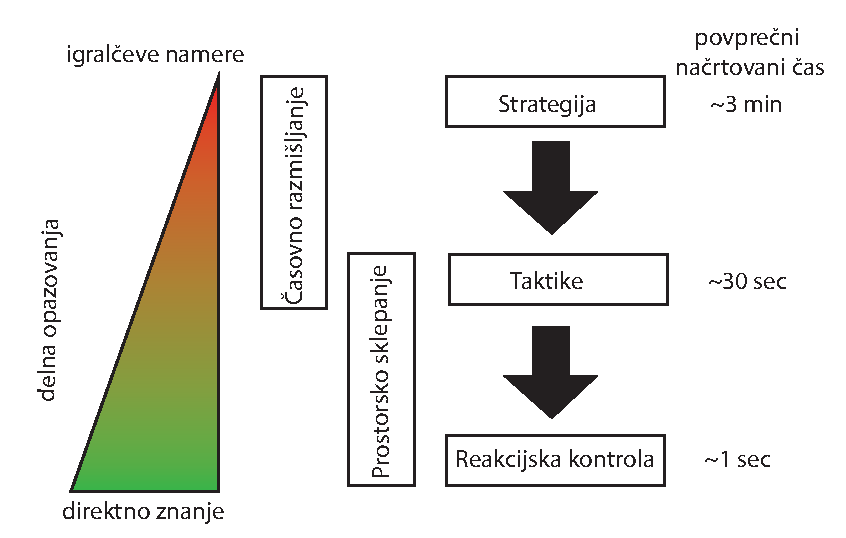
\includegraphics[width=0.6\textwidth]{RazdelitevNalog.pdf}
		\end{center}
		\caption{Razdelitev nalog.}
		\label{pic1}
	\end{figure}
	
	Pogosto razdelimo odločanje na dva dela:
	\begin{itemize}
		\item Micro, kjer kontroliramo enote posamezno
		\item Macro, kjer se osredotočimo na ekonomijo in izdelavo enot
	\end{itemize}
\end{itemize}

\section{Strategija}
V strateških igrah je velikokrat uporabljen pristop direktnega kodiranja strategije, ki uporabljajo avtomate končnih stanj, kjer lahko razbijemo delovanje na več stanj kot so napadanje, nabiranje surovin, popravilo itd. in hitro menjavanje med njimi. Direktno kodiranje prinese dobre pričakovane rezultate, vendar se lahko igralec nauči strategije in ga tako agenta hitro porazi.
Planirani pristopi ponujajo večjo prilagodljivost kot direktno kodirani.
\section{Taktika}
Taktika spada pod direktnejši nadzor enot kakor strategija in je bolj osredotočena na kontrolo določenih točk na mapi, zmagi posameznih bitk in iskanje ožin, kjer je nasprotnik šibkejši. Taktika temelji na analizi terena, ki ga lahko razbijemo na kompozicijo ožin.

\section{Abstrakcija prostora}
tle napišeš kok je to komplex k maš strategije pa da rabš ful abstractat če bi hotu strategijo razbrat najbolšo, pa taktiko
Pa če maš fog of war maš probleme
Prav tako je pa tu problem, da je StarCraft le delno viden, kjer le del algoritmov deluje ob nevednosti nasprotnikovih akcij.



\chapter{Predstavitev algoritma Alpha Zero}
\label{alphazero}
Zakaj je dobr algoritem pa zakaj sem ga izbral za rts igro
\section{Zgodovina}
However, AlphaGo (Silver et al. 2016), which uses recent deep reinforcement learning and Monte Carlo Tree Search methods, managed to defeat the top human player, through extensive use of domain knowledge and training on the games played by top human players~cite{silver2016mastering}.

Recently, however, AlphaGo Zero (Silver et al. 2017b) described an approach that used absolutely no expert knowledge and was trained entirely Stanford University CS238 Final Project Report through self-play. This new system, AlphaGo Zero, even outperforms the earlier AlphaGo model. This represents a very exciting result, that computers may be capable of superhuman performances entirely through self-learning, and without any guidance from humans~cite{silver2017mastering}.


Pa da je zdj alpha zero ker se uči sam prot seb. mogoče daš kšne reference z googla


TODO - napiš zakaj je pristop samostojnega učenja najprimernejši
\section{Potek učenja}
Napišeš da se uči sam prot seb, pa da uporabla mcts za iskanje. Napišeš mcts zato ker je preiskovalni prostor prevelik

TOLE MAŠ REFERENCAN:
https://arxiv.org/pdf/1712.01815.pdf \\

AlphaZero learns these move probabilities and value estimates entirely from selfplay;
these are then used to guide its search.
Instead of an alpha-beta search with domain-specific enhancements, AlphaZero uses a generalpurpose
Monte-Carlo tree search (MCTS) algorithm. Each search consists of a series of simulated
games of self-play that traverse a tree from root sroot to leaf. Each simulation proceeds by
selecting in each state s a move a with low visit count, high move probability and high value
(averaged over the leaf states of simulations that selected a from s) according to the current
neural network fo. The search returns a vector pi representing a probability distribution over
moves, either proportionally or greedily with respect to the visit counts at the root state.
The parameters o of the deep neural network in AlphaZero are trained by self-play reinforcement
learning, starting from randomly initialised parameters o. Games are played by selecting
moves for both players by MCTS, at ∼ rt
. At the end of the game, the terminal position sT is
scored according to the rules of the game to compute the game outcome z: −1 for a loss, 0 for
a draw, and +1 for a win. The neural network parameters o are updated so as to minimise the
error between the predicted outcome vt and the game outcome z, and to maximise the similarity
of the policy vector pt
to the search probabilities rt
. Specifically, the parameters o are adjusted
by gradient descent on a loss function l that sums over mean-squared error and cross-entropy
losses respectively,



\section{Končno število potez}
Napišeš kok so igre na katerih dela to preproste - pa da so 2 barvi. pa pač da moj game


\chapter{Definiranje pravil igre}
\label{chpravilaigre}

Igro smo definirali po Surag Nairjevi predlogi za Alpha Zero, ki je na voljo na (portalu?) Github (Insert reference here).
Igra je dodana kot modul, ki vsebuje definicijo igre in njena pravila, igralce, vizualizacijo in izgradnjo modela




Igra je definirana v kvadratni mreži 8x8, kjer polje lahko vsebuje največ eno figuro.
Ostale igre, ki so napisane za to različico Alpha Zero izvedbe, kot na primer štiri v vrsto, gobang, othello, tri v vrsto, vsebujejo črno-bele figure.
Zakodirane so lahko z eno številko: -1 za igralca -1, +1 za igralca +1 ali 0, če je polje prazno.
Pri rts igrah pa moramo vedeti poleg igralca, komur ta figura pripada, tudi stanje te figure, na primer trenutno zdravje in tip figure.
Zato je prostor kodiranja 3-dimenzionalen in ne 2. Več o kodiranju stanj v (insert section here)

Board is presented as 3D integer array of dimensions width, height, 6 (which represents number of properties in Tile encoding)

\section{Actors}
\subsection{Actor types}


Gold - Resource source unit
Worker - Unit that can gather, return resources and build all types of buildings
Barracks - Building that can build units of type Rifle Unit
Rifle Unit - Units that can attack enemy units
Town Hall - Building that produces Worker units

\subsection{Actions}

idle: Pass turn
up: Move up 1 field if its empty
down: Move down 1 field if its empty
right: Move right 1 field if its empty
left: Move left 1 field if its empty
naberi zlato: Mine gold resources if standing nearby
vrni zlato: Return gold resources if carrying gold to Town Hall
attack: Attack nearby unit
npc: Build worker character
vojak: Build attack unit
barracks: Build building that produces attacking units
glavna hiša: Build building that produces workers and is resource deposit

\subsection{Tile Encoding}
Tile encoding

Each actor is encoded using following 6 properties:

Player Name: [-1,0,1] (player -1, empty field, player 1)
Actor Type: [1-5] Numerically encoded Actor Type of written above
Health: [1-31] Current actor health - when actor has 0 health, it gets destroyed
Carry: [0,1] If Worker unit is carrying resources or not - it gets set when worker uses mine resources near resource source and gets removed when worker uses return resources near resources drain actor.
Money: [0-*] Current amount of money that this player has at current time (When money updates, it updates on every players actor)
Time: [*-0 or 0-8191] Countdown time that gets updated on every board tile when move gets executed. Also timer that increases, and special milestones, health is decreased for all units by formula.


\section{Akcije}

Opišeš vse akcije, 
opišeš da si idle removov, 



\subsection{Action checking sequence
}
Following actions are checked and executed in some order:

\begin{itemize}
	\item naberi zlato
	\item vrni zlato
	\item napadi
	\item delavec
	\item vojak, 
	\item vojašnica
	\item glavna hiša
\end{itemize}
\begin{verbatim}
coords = [(x - 1, y + 1),
          (x, y + 1),
          (x + 1, y + 1),
          (x - 1, y),
          (x + 1, y),
          (x - 1, y - 1),
          (x, y - 1),
          (x + 1, y - 1)]
for n_x, n_y in coords:
    # check action condition or execute action
\end{verbatim}
When first tile is free in these coordinates, building or unit is spawned there.
When first enemy in this tile sequence is chosen, it is attacked.
This results in building units and buildings towards lower-left corner, as units progress towards x-1, y+1 as this tile is free, expanding towards upper-right corner only when all other options are used.

Fix for this would be to make actions for each of these coordinates for each of actions that use them, resulting in much higher action space






\section{Kodiranja}
opišeš za maxhealth, cost, .... lah nardiš tabelce pa use to notr vržeš



Figuro zakodiram z naslednjimi stanji:
\begin{itemize}
	\item Ime igralca: 
	\item Tip figure:
	\item Trenutno zdravje figure:
	\item Nosi zlato:
	\item Denar:
	\item Čas igranja:
\end{itemize}


\begin{table}
	\begin{center}
		
	\begin{tabular}{p{0.2\linewidth}|p{0.4\linewidth}|p{0.2\linewidth}|p{0.2\linewidth}}
		Ime figure & {\tt Akcije} & {\tt Zdravje} & {\tt Strošek izdelave} \\ \hline
		{\tt Zlato} & / & 10 & 0 \\
		{\tt Delavec}   & gor, dol levo desno, vojašnica, glavna hiša, naberi zlato, vrni zlato, zdravi & 10  & 1 \\
		{\tt Vojašnica}   & vojak, zdravi & 10  & 4 \\
		{\tt Vojak}   & gor, dol, levo, desno, napad, zdravi  & 20 & 2 \\
		{\tt Glavna hiša}   & delavec, zdravi & 30  & 7 \\
	\end{tabular}


	\end{center}
	\caption{}
	\label{tbl:1}
\end{table}


\subsection{Desetiško kodiranje}
Dimenzija zakodiranega prostora je tako 8x8x6

\subsection{One Hot kodiranje}
\begin{itemize}
	\item Ime igralca: 2 bit - 00(neutral), 01(1) or 10(-1),
	\item Tip figure: 4 bit,
	\item Trenutno zdravje figure: 5 bit,
	\item Nosi zlato: 1 bit,
	\item Denar:  5 bits (32 aka 4 town halls or 32 workers) [every unit has the same for player]
	\item Čas igranja: 2 na 13 8192(za total annihilation)
\end{itemize}
Dimenzija zakodiranega prostora je tako 8x8x13

\section{Konec igre}

Instance of game is finished in following conditions:

One of players does not have any available moves left (board is populated or one player is surrounded),
One players' actors get destroyed,
When remaining time reaches 0


\section{Izluščevanje učnih primerov}
To nardiš z get symmetries
\section{Reševanje problema neskončnega števila potez}
Tukej napišeš za time killer krivulje ter heal funkcijo



\section{Initial board configuration}
Board gets setup with a town hall for each player in the middle, with 2 patches of resource source actor - Minerals. Each mineral patch is assigned its player (-1,1), because value 0 game recognises as unpopulated area. Each player then starts with some amount of gold (1 or 20 or 100...).

Slika~\ref{destroy_formula_2018_10_20} je v {\tt .pdf} formatu.
\begin{figure}[h]
	\begin{center}
		\includegraphics[width=0.8\textwidth]{destroy_formula_2018_10_20.pdf}
	\end{center}
	\caption{Herschelov graf, vektorska grafika. Os x ne prikazuje celotnega zajema časa igre (8192).}
	\label{destroy_formula_2018_10_20}
\end{figure}
Blue curve represents how much damage is dealt to specific unit in given game time. Red curve represents how many actors have been damaged in current time frame.

We can see that Damage curve is far more strict and is beginning to rise quite early in the game. That's because we want to quickly eliminate non-working player instances and prioritize those that are collecting minerals and spawning new actors. We can also see y axis span from 0 to 64, which is maximum total of actors for one player, so at round ~8000, every actor on board will recieve fatal damage, so timeout is never reached.

Actors can also heal each other using money, so they can prolong their life.


\chapter{Učenje modela}
\label{chucenjemodela}
Learning of this game is complicated, because of end game conditions. Learning wrapper expects game to finish using MCTS simulations, but python might run into max recursion depth exceeded exception, because player is repeating same move multiple times.
This can be solved using timeouts, as where simulation gets stopped when we run out of remaining moves, but can lead to inaccurate MCTS tree, because nodes do not get properly evaluated during backpropagation.
Proper end condition must be found or change of source is needed in order to exclude timeouts, because they are not returning best resuts.


Possible learning idea
Idea is to incrementally learn model by changing end game condition. First start learning model on simple end game condition like producing workers and when model is successfully creating workers, add another condition on top of that already learnt model.
Possible problem might occur because of model size



\section{TensorFlow}

Keras je module tensorflowa


formula po kateri računa

\begin{izrek}
	\label{iz:1}
	Za vsako naravno število $n$ velja
	\begin{equation}
	R(s,a) = Q(s,a) + cpuctP(s, a)\sqrt{\dfrac{\sum{b}*N(s,b)}{N(s,a)}}
	\label{eq:1}
	\end{equation}
\end{izrek}


Opišeš parameter mcts sims in cpuct, arenacompare, numiters, numeps, 






\chapter{Vizualizacije}
\label{chvizualizacija}

\section{Pygame}
napišeš daj to ez vizualizacija za pregled igre med kodiranjem, pa da če human igra lah interacta s keyboardom al pa miško
Pa napišeš da prkazuješ v gridu s krogci, pa maš flage pa pozete k so možne


Pri vizualizaciji s Python knjižnico Pygame, lahko uporabnik nadzoruje svoje figure s tipkovnico in miško.

Uporabnik mora najprej izbrati figuro z levim miškinim klikom in potem izbrati določeno akcijo, ki je izpisana na zaslonu. Uporabnik lahko spremeni figuro, tako da jo odznači s klikom desnega miškinega gumba na prazno mesto.


Moving: User can move workers and infantry by 1 square in all 4 directions if they are empty by clicking on one of 4 corresponding tiles.
Attacking: With selected infantry unit, user can attack enemy units that are in range.
Gathering and returning resources: With worker selected, user can mine resources by clicking right mouse button on Gold actor if in range. This goes the same when returning resources, but worker must be nearby Town Hall actor.
Building: For building units and buildings, user must use one of keyboard shortcuts written on canvas.
Idle: User can press space to idle with selected actor.

Console:
Type one of listed commands seperated by space and press Enter.

Slika~\ref{visualization_pygame} je v {\tt .pdf} formatu.
\begin{figure}[h]
	\begin{center}
		\includegraphics[width=0.8\textwidth]{visualization_pygame.pdf}
	\end{center}
	\caption{Herschelov graf, vektorska grafika.}
	\label{visualization_pygame}
\end{figure}

\section{Unreal Engine 4}

Unreal Engine 4 je odprtokodni program podjetja Epic Games, ki je namenjen hitri izdelavi računalniških iger. Obstajajo še drugi celostni pogoni kot je Unity.\\
Razliko med tema pogonoma je dobro predstavil Marko Kladnik \cite{diploma2}.\\
Unreal Engine 4 omogoča hitro ustvarjanje iger s pomočjo posebnih diagramov (angl. blueprint) in hkrati podpira programski jezik C++, ki ga uporabimo za hitro izvedbo velikega števila matematičnih izrazov.\\

Potrebno je bilo preslikati akcije in figure v urejevalnik Unreal Engine, da se tam enote primerno premikajo in izvajajo akcije.
Potrebno je bilo mapirati animacije, efekte, da premikanje in napadanje zgleda dokaj realistično.

Ta predstavitev omogoča tudi igranje dveh človeških igralcev enega proti drugemu preko internetne mreže, kjer vsak igralec pridobiva priporočene ukaze iz modela.
Človeški igralec lahko igra tudi proti računalniškim igralcem, ki pa vsaki 2 sekundi zahteva za novo najboljšo akcijo.
Lahko si pa ogledamo dva računalniška igralca igrati drug proti drugemu.


Slika~\ref{visualization_ue4} je v {\tt .pdf} formatu.
\begin{figure}[h]
	\begin{center}
		\includegraphics[width=0.8\textwidth]{visualization_ue4.pdf}
	\end{center}
	\caption{Herschelov graf, vektorska grafika.}
	\label{visualization_ue4}
\end{figure}


\subsection{Prenos stanja igre}
napišeš kko encodaš game pa ga pošleš pythonu, tm pa dobiš best action pa pol nazaj...


\chapter{Rezultati}
\label{chrezultati}
Opišeš parametre in čas učenja
Opišeš rezultate pri različnih nastavitvah parametru igre - recmo bolj stroga krivulja, manj stroga, več denarja per mine, cenejši heal...
Pa s kermu encodingom so bli bolši razultati
Pa napišeš primerjava proti naključnim igralcem in greedy- kjer ima greedy player kriterij za število življenja maximize
\section{Učenje s prekinitvijo časa}
\section{Učenje z ranjujočo funkcijo}


\chapter{Zaključek}
\label{chzakljucek}
Ali se to splača za moderni rts game- NE! :D
kje je problem -> v prostoru, v pristopu z koncem igre


Igra je na voljo na naslednjih repozitorijih:
https://github.com/JernejHabjan/TrumpDefense2020
https://github.com/JernejHabjan/alpha-zero-general


\newpage %dodaj po potrebi, da bo številka strani za Literaturo v Kazalu pravilna!
\ \\
\clearpage
\addcontentsline{toc}{chapter}{Literatura}
\bibliographystyle{plain}
\bibliography{literatura}


\end{document}

